\documentclass[CJKmath,10pt,a4paper]{exam-zh}

\examsetup{
	page/size=a4paper,
	paren/show-paren=true,
	paren/show-answer=true,
	fillin/show-answer=false,
	solution/show-solution=show-stay,
	solution/label-indentation=false,
	page/show-head=true,
	page/foot-content=\textbf{物理习题}\ 第;/;页,
}
% 若〈页脚格式〉中不含西文分号;，则页脚内容为〈页脚格式〉直接输出；
% 若〈页脚格式〉中含一个西文分号;，如foo;bar，则页脚为foo<the page>bar，即西文分号代替了页码的位置；
% 若〈页脚格式〉中含两个西文分号;，如foo;bar;baz，则页脚为foo<the page>bar<total page>baz，即第一个西文分号代替了页码的位置，第二个代替了总页码

\usetikzlibrary{calc}
%\usepackage{yhmath}
\begin{document}



\section{%  
竖直圆与机械能
}

\begin{question}
如图所示，绝缘水平面上固定一光滑绝缘的竖直圆弧轨道 \(BCD\)，圆心为 $O$，$C$ 点与圆心等高，$B$ 点为圆弧轨道与水平面的切点，$D$ 点为轨道的末端，$OD$ 与水平方向的夹角 $\theta=37^\circ$，圆弧轨道半径 $R=1.0\text{m}$。质量 $m=0.4\text{kg}$、电荷量 $q=+0.03\text{C}$ 的滑块静止在 $A$ 点。某时刻在整个空间加上水平向左的匀强电场，电场强度 $E=100\text{N/C}$，滑块开始运动。已知 $A$、$B$ 间的水平距离 $x_{AB}=3.6\text{m}$，滑块与水平面间的动摩擦因数 $\mu=0.25$，重力加速度 $g$ 取 $10\text{m/s}^2$，取 $\sin37^\circ=0.6$，规定 $B$ 点电势为零，滑块可视为质点。求：

\begin{enumerate}
	\item 滑块在圆弧轨道上的最小电势能；
	\item 滑块在圆弧轨道上运动时，滑块对轨道的最大压力大小；
	\item 	滑块第三次经过 $B$ 点时的速度大小。
\end{enumerate}
% --- 图形绘制部分 ---
\begin{center}
	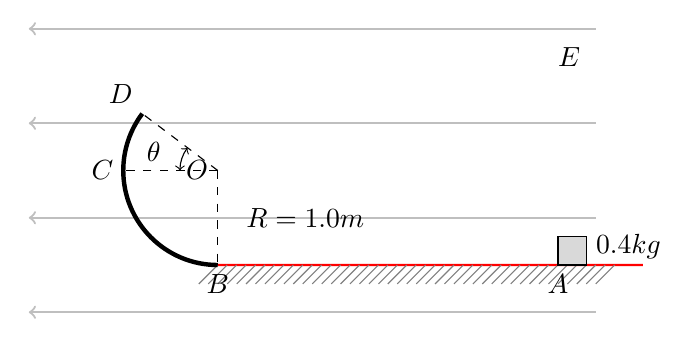
\begin{tikzpicture}[scale=1.2]
		% 定义坐标
		\coordinate (O) at (0,0); % 圆心
		\coordinate (B) at (0,-1); % B点 (切点)
		\coordinate (C) at (-1,0); % C点 (与圆心等高)
		% D点: OD与水平方向夹角37度，位于第二象限
		% x = -cos(37), y = sin(37)
		\coordinate (D) at ({-cos(37)}, {sin(37)});
		\coordinate (A) at (3.6, -1); % A点 (距离B点3.6m)
		
		% 1. 绘制电场线 (背景)
		\foreach \y in {-1.5, -0.5, 0.5, 1.5} {
			\draw[->, gray!50, thick] (4, \y) -- (-2, \y);
		}
		
		% 2. 绘制地面 (水平线)
		\draw[thick,red] (B) -- (4.5, -1);
		% 地面阴影
		\foreach \x in {0,0.1, ..., 4.3} {
			\draw[gray] (\x, -1) -- (\x-0.2, -1.2);
		}
		
		% 3. 绘制圆弧轨道 BCD
		% 从B点(270度) 到 D点(180-37 = 143度)
		\draw[ultra thick] (B) arc[start angle=270, end angle={180-37}, radius=1];
		
		% 4. 绘制辅助虚线
		\draw[dashed] (O) -- (B); % OB
		\draw[dashed] (O) -- (C); % OC (虽然重合在轴上，画出来明确一下)
		\draw[dashed] (O) -- (D); % OD
		
		% 5. 绘制滑块 (在A点)
		\draw[fill=gray!30] (A) rectangle ++(0.3, 0.3);
		\node[right] at (3.9, -0.8) {$0.4\text{kg}$}; % 标注质量
		
		% 6. 标注点和角度
		\node[left] at (O) {$O$};
		\node[below] at (B) {$B$};
		\node[left] at (C) {$C$};
		\node[above left] at (D) {$D$};
		\node[below] at (A) {$A$};
		
		% 角度标注
		\draw[<->] (-0.4, 0) arc[start angle=180, end angle={180-37}, radius=0.4];
		\node[left] at (-0.5, 0.2) {$\theta$};
		
		% 半径标注
		\node[right] at (0.2, -0.5) {$R=1.0\text{m}$};
		
		% 电场强度标注
		\node[right] at (3.5, 1.2) {$E$};
		
	\end{tikzpicture}
\end{center}
\end{question}	
\begin{solution}
解题分四步进行。\par

第1步：求滑块第一次到达 $B$ 点时的速度。\par
滑块在水平面 $AB$ 上受水平向左的电场力
\[
F_e=qE=0.03\times 100=3\text{ N}
\]
受滑动摩擦力
\[
f=\mu mg=0.25\times 0.4\times 10=1\text{ N}
\]
从 $A$ 到 $B$ 过程中，由动能定理得
\[
(F_e-f)x_{AB}=\frac12 mv_{B1}^2
\]
代入数据：
\[
(3-1)\times 3.6=\frac12\times 0.4\times v_{B1}^2
\]
解得
\[
v_{B1}=6\text{ m/s}
\]

第2步：建立滑块在圆弧轨道上任意位置的速度表达式。\par
设滑块在圆弧上某点 $P$ 时，$\angle BOP=\varphi$。则该点相对 $B$ 点升高的高度为
\[
h=R(1-\cos\varphi)
\]
相对 $B$ 点的水平坐标为
\[
x=-R\sin\varphi
\]
规定 $B$ 点电势为零，则该点的电势能为
\[
E_p=qEx=-qER\sin\varphi=-3\sin\varphi\text{ J}
\]
重力势能为
\[
E_g=mgh=mgR(1-\cos\varphi)=4(1-\cos\varphi)\text{ J}
\]
圆弧轨道光滑，机械能守恒：
\[
\frac12 mv^2+4(1-\cos\varphi)-3\sin\varphi=\frac12 m v_{B1}^2=7.2
\]
整理得
\[
0.2v^2=3.2+4\cos\varphi+3\sin\varphi
\]
即
\[
v^2=16+20\cos\varphi+15\sin\varphi
\]

第(1)问：滑块在圆弧轨道上的最小电势能。\par
由
\[
E_p=-3\sin\varphi
\]
可知，当 $\sin\varphi$ 最大时，电势能最小。圆弧上最靠左的位置为 $C$ 点，此时 $\varphi=90^\circ$，故
\[
E_{p\min}=-3\text{ J}
\]

第(2)问：滑块对轨道的最大压力。\par
先判断滑块能否到达 $D$ 点。由题意，$OD$ 与水平方向夹角为 $37^\circ$，故在 $D$ 点有
\[
\sin\varphi_D=\cos37^\circ=0.8,\qquad \cos\varphi_D=-\sin37^\circ=-0.6
\]
代入上式得
\[
v_D^2=16+20\times(-0.6)+15\times 0.8=16
\]
所以
\[
v_D=4\text{ m/s}
\]
说明从能量角度看，滑块可以到达 $D$ 点。\par

再判断到达 $D$ 点前是否会脱离轨道。设轨道对滑块的支持力为 $N$，沿指向圆心方向列牛顿第二定律：
\[
N-mg\cos\varphi-qE\sin\varphi=\frac{mv^2}{R}
\]
故
\[
N=\frac{mv^2}{R}+mg\cos\varphi+qE\sin\varphi
\]
在 $D$ 点代入数据得
\[
N_D=0.4\times 16+4\times(-0.6)+3\times 0.8=6.4\text{ N}>0
\]
因此滑块到达 $D$ 点时仍与轨道保持接触，不会提前脱轨，所以\textbf{滑块能够到达 $D$ 点}。\par

下面求最大压力。将
\[
v^2=16+20\cos\varphi+15\sin\varphi
\]
代入支持力表达式：
\[
N=0.4(16+20\cos\varphi+15\sin\varphi)+4\cos\varphi+3\sin\varphi
\]
整理得
\[
N=6.4+12\cos\varphi+9\sin\varphi
\]
又因为
\[
12\cos\varphi+9\sin\varphi=15(0.8\cos\varphi+0.6\sin\varphi)
\]
所以
\[
N=6.4+15(\cos\varphi\cos37^\circ+\sin\varphi\sin37^\circ)
\]
即
\[
N=6.4+15\cos(\varphi-37^\circ)
\]
当 $\varphi=37^\circ$ 时，$N$ 取最大值，故
\[
N_{\max}=6.4+15=21.4\text{ N}
\]
由牛顿第三定律，滑块对轨道的最大压力大小也为
\[
21.4\text{ N}
\]

第(3)问：滑块第三次经过 $B$ 点时的速度大小。\par
滑块第一次经过 $B$ 点后沿圆弧运动，到达 $D$ 点时速度仍不为零。此时它离开轨道后并不是通常的斜上抛运动，因为它仍同时受到重力和水平向左的电场力。\par
在 $D$ 点，滑块速度方向沿轨道切线向右上方；而电场力向左、重力向下，它们的合力方向为左下方。由题给三角关系可知，这个合力方向恰好与 $D$ 点的速度方向相反，所以滑块离开 $D$ 点后做匀减速直线运动，速度减为零后再沿原直线返回 $D$ 点。\par
由于圆弧轨道光滑，滑块从 $D$ 返回到 $B$ 的过程中机械能守恒，所以第二次经过 $B$ 点时速度仍为
\[
v_{B2}=6\text{ m/s}
\]

第二次经过 $B$ 点后，滑块向右进入粗糙水平面。此时电场力向左、摩擦力也向左，总阻力大小为
\[
F'=3+1=4\text{ N}
\]
设它向右滑行的最大距离为 $s$，由动能定理得
\[
4s=\frac12\times 0.4\times 6^2=7.2
\]
解得
\[
s=1.8\text{ m}
\]
由于 $1.8\text{ m}<3.6\text{ m}$，所以滑块不会回到 $A$ 点，而是在 $AB$ 间某处停止后再向左运动。\par

从静止点返回 $B$ 的过程中，电场力向左，摩擦力向右，合力大小为
\[
F''=3-1=2\text{ N}
\]
因此合力做功为
\[
W=F''s=2\times 1.8=3.6\text{ J}
\]
由动能定理，第三次经过 $B$ 点时
\[
\frac12 mv_{B3}^2=3.6
\]
即
\[
\frac12\times 0.4\times v_{B3}^2=3.6
\]
解得
\[
v_{B3}=3\sqrt{2}\text{ m/s}
\]

综上：
\[
\boxed{E_{p\min}=-3\text{ J}}
\]
\[
\boxed{N_{\max}=21.4\text{ N}}
\]
\[
\boxed{v_{B3}=3\sqrt{2}\text{ m/s}}
\]
\end{solution}


\end{document}